Typically, a computational campaign for drug discovery explores a large
number of drug candidates by running several workflows multiple times, each
requiring thousands of concurrent simulations. Before embarking on a campaign
that will utilize 150 million core hours on NCSA Blue Waters, we perform
experiments to characterize the weak and strong scaling performance of HTBAC
and its overheads on Blue Waters. We validate the results of the free energy
calculations produced using HTBAC against published results.

Given that protocols like TIES are more computationally demanding than
protocols like ESMACS, it is paramount to use resources efficiently,
especially for campaigns that have a predefined computational budget. As
described in \S~\ref{sec:science-drivers} and~\ref{sec:htbac}, adaptive
simulation methods have the potential to reduce the number of simulations
without a loss in accuracy and with a lower computational load. We run
experiments with an adaptive implementation of TIES in HTBAC, measuring the
benefits in terms of accuracy, reduced number of simulations and
computational load.

% A -------------------------------------------------------------------------
\subsection{Experiment Setup}\label{ssec:exp_design}

Table~\ref{tab:experiments} shows 9 experiments we designed to characterize
the behavior of HTBAC on Blue Waters. Each experiment executes the ESMACS
and/or TIES protocol for different physical systems. Experiments 1--6 use the
BRD4 physical system provided by GlaxoSmithKline, while experiments 7--9
utilize the PTP1B, MC1, and TYK2 physical systems.

\begin{table*}
    \caption{Parameters of scalability and adaptivity
    experiments.}\label{tab:experiments}
    \centering
    \begin{tabular}{l                    % Experiment ID
                    l                    % experiment type
                    l                    % physical system 
                    l                    % protocol type
                    l                    % number of protocols
                    l                    % total cores
                    }
    %
    \toprule
    %
    \B{ID}                            &  % Experiment ID
    \B{Type of Experiment}            &  % experiment type
    \B{Physical System(s)}            &  % physical system
    \B{Protocol(s)}                   &  % protocol type
    \B{No. Protocol(s)}               &  % number of protocols
    \B{Total Cores}                   \\ % total cores
    %
    \midrule
    %
    \B{1}                             &  % Experiment ID
    Weak scaling                      &  % experiment type
    BRD4                              &  % physical system
    ESMACS                            &  % protocol type
    (2, 4, 8, 16)                     &  % number of protocols
    1600, 3200, 6400                  \\ % total cores
    % 
    \B{2}                             &  % Experiment ID
    Weak scaling                      &  % experiment type
    BRD4                              &  % physical system
    TIES                              &  % protocol type
    (2, 4, 8)                         &  % number of protocols
    4160, 8320, 16640                 \\ % total cores
    %
    \B{3}                             &  % Experiment ID
    Weak scaling                      &  % experiment type
    BRD4                              &  % physical system
    ESMACS + TIES                     &  % protocol type
    (2, 4, 8)                         &  % number of protocols
    5280, 10560, 21120                \\ % total cores
    %
    \B{4}                             &  % Experiment ID
    Strong scaling                    &  % experiment type
    BRD4                              &  % physical system
    TIES                              &  % protocol type
    (8, 8, 8)                         &  % number of protocols
    16640, 8320, 4160                 \\ % total cores
    %
    \B{5}                             &  % Experiment ID
    Strong scaling                    &  % experiment type
    BRD4                              &  % physical system
    ESMACS                            &  % protocol type
    (16, 16, 16)                      &  % number of protocols
    6400, 3200, 1600                  \\ % total cores
    %
    \B{6}                             &  % Experiment ID
    Strong scaling                    &  % experiment type
    BRD4                              &  % physical system
    ESMACS + TIES                     &  % protocol type
    (20, 20, 20)                      &  % number of protocols
    22120, 10560, 5280                \\ % total cores
    %
    \B{7}                             &  % Experiment ID
    Non-adaptivity                    &  % experiment type
    PTP1B, MC1, TYK2                  &  % physical system
    TIES                              &  % protocol type
    (1, 1, 1)                         &  % number of protocols
    2080, 2080, 2080                  \\ % total cores
    %
    \B{8}                             &  % Experiment ID
    Adaptivity                        &  % experiment type
    PTP1B, MC1, TYK2                  &  % physical system
    TIES                              &  % protocol type
    (1, 1, 1)                         &  % number of protocols
    2080, 2080, 2080                  \\ % total cores
    %
    \B{9}                             &  % Experiment ID
    Reference                         &  % experiment type
    PTP1B, MC1, TYK2                  &  % physical system
    TIES                              &  % protocol type
    (1, 1, 1)                         &  % number of protocols
    10400, 10400, 10400               \\ % total cores
    %
    \bottomrule
    %
    \end{tabular}
\up{}
\end{table*}

Experiment 1 and 2 measure the weak scaling of HTBAC using the ESMACS and
TIES protocols. Experiments 3 uses both the TIES and ESMACS protocols,
characterizing the weak scaling of heterogeneous protocol executions.
Experiments 4 and 5 measure the strong scaling of HTBAC using a fix number of
instances of the ESMACS and TIES protocols. Experiments 6 uses both the TIES
and ESMACS protocols, characterizing the strong scaling of heterogeneous
protocol executions. Experiments 7--9 characterize nonadaptive and adaptive
simulation methods using the TIES protocol.

In each weak scaling experiment (1--3), we keep the ratio between resources
allocated and protocol instances constant. Consistently, for each experiment
we progressively increase both the number of cores (i.e., measure of
resource) and the number of protocol instances by a factor of 2. In each
strong scaling experiment (4--6), we change the ratio between resources
allocated and the number of protocol instances: we fix the number of protocol
instances and reduce the number of cores by a factor of 2.

Weak scaling experiments provide insight into the size of the workload that
can be executed in a given amount of time, while strong scaling experiments
show how the time duration of the workload scales when adding resources. For
all the weak and strong scaling experiments we characterize the overheads of
HTBAC, EnTK and RP, and we show an approximation of the time taken by the
resources to become available. This offers insight about the impact of HTBAC
and its runtime system on the time to completion of each workload.
In~\cite{dakka2017}, we show baseline performance of HTBAC using ESMACS with
a null workload.

For weak and strong scaling experiments, we reduced the number of time-steps
of the protocols and omitted the analysis steps $S5$ and $S6$ of their
workflows (Fig.~\ref{fig:ties_esmacs_application}). These simplifications are
consistent with characterizing scalability performance instead of simulation
duration. The time-steps are set to enable enough time for load balancing of 
the physical system to complete. For the experiments 1--6 we used the following 
time-steps: $S1=1000$; $S2=5000$; $S3=5000$; and $S4=50000$.

We measure the following durations for Experiments 1--6:
\begin{itemize}
    \item \textbf{Total Task Execution Time}: Time taken by all the task
    executables to run on the computing infrastructure.
    \item \textbf{HTBAC Overhead}: Time taken to instantiate HTBAC, and
    validate and process the application description.
    \item \textbf{EnTK and RP Overhead}: Time taken by EnTK and RP to manage
    the execution of tasks.
    \item \textbf{\texttt{aprun} Overhead}: Time taken by \texttt{aprun} to
    launch tasks on Blue Waters.
\end{itemize}

Note that once RP relinquishes the control flow to \texttt{aprun}, the
precise time at which \texttt{aprun} schedules each task on a compute node
and the MD kernel of each task begins execution cannot be measured. Instead,
for each task, we measure the difference between the task execution time and
its \texttt{NAMD} kernel execution time, provided by the \texttt{NAMD} output
logs. In this way, we approximate the time taken by \texttt{aprun} to launch
the task. Once aggregated, these measures constitute what we defined as
\texttt{aprun} Overhead. The summation of all durations provides the average
wall-time of the pilot job.

Experiments 7--9 compare the accuracy and time to solution of nonadaptive and
adaptive simulation methods. For the nonadaptive simulation method of
Experiment 7 we use 13 preassigned and approximated $\lambda$ windows,
consistent with the value reported in Ref.~\cite{Bhati2017}. In this way, we
produce 65 concurrent simulations for stages $S1$--$S4$ of TIES (see
Fig.~\ref{fig:ties_esmacs_application}). The production simulation stage $S4$
executes each simulation for \SI{4}{\nano\second}. Stage $S5$ has 5 analysis
tasks which aggregate the simulation results of $S4$. The global analysis
stage $S6$ has a single task that aggregates the results from $S5$.

In the adaptive implementation~\ref{fig:adaptive_TIES}, we initialize the
TIES protocol with 3 $\lambda$ windows, obtaining 15 replicas. We separate
stage $S4$ of each TIES replica into 4 sub-stages. Each sub-stage runs a
\SI{1}{\nano\second} simulation, followed by an adaptive quadratures analysis
which estimates free energy errors with respect to each interval of two
$\lambda$ values.

We use Experiment 9 to compare the adaptive and non-adaptive execution of
TIES. We use % a large number of (65) 
65 simulations, derived from 13 equally spaced $\lambda$ windows to calculate
the free energy with high accuracy. This creates a baseline against which to
compare the adaptive and non-adaptive results.

\begin{figure}
  \centering
  \includegraphics[width=\columnwidth]{figures/Adaptive_TIES.pdf}
  \caption{Adaptive workflow for TIES. After equilibrating 3 $\lambda$, the
  first stage starts. This is followed by analysis at every $\lambda$
  interval, to decide whether to add a new window in between. In our
  implementation, the simulation-analysis cycle is repeated for 4 simulation
  steps, not shown here.}\label{fig:adaptive_TIES}
\up{}
\up{}
\up{}
\end{figure}

We assigned the following simulation time-steps in Experiment 7 and 9:
$S1=3000$; $S2=50000$; $S3=50000$; and $S4=2000000$. The adaptive simulation
of Experiment 8 uses the same time-steps, apart from $S4$ which is divided
into 4 sub-stages of 500000 time-steps each.

We performed all the experiments on Blue Waters, a 26868 node Cray XE6/XK6
SuperComputer with peak performance of 13.3 petaFLOPS managed by NCSA.
consistent with NCSA policies, we initiated the experiments from a virtual
machine outside NCSA, avoiding to run persistent process on the NCSA login
node. We used HTBAC 0.1, EnTK 0.6, and RP 0.47 and the \texttt{NAMD-MPI} MD
kernel, and launched via the \texttt{aprun} command. For the analysis stages
in the TIES protocol we used \texttt{AmberTools}.

NCSA sets a system policy on the maximum number of processes that
\texttt{aprun} can spawn, limiting the number of concurrent tasks we can
execute on Blue Waters to $\approx$450. During the execution of Experiment 2,
we observed failing tasks with 8 TIES protocol instances, i.e., 520
concurrent tasks. In a trial of 10 repetitions at this scale, we observed an
average of $70\pm6.67$ failing tasks. More data would be required to model
the distribution type of these results.

NCSA allows to run only one MPI application for each compute node. Thus, we
run each MD simulation with 32 cores (i.e., one compute node) even if our
performance of \texttt{NAMD} on Blue Waters indicated that 16 cores offers
the best trade-off between computing time and communication overhead.

% B -------------------------------------------------------------------------
\subsection{Weak Scaling Characterization}

Fig.~\ref{fig:ws}(a) shows the weak scaling of HTBAC with the TIES protocol.
Each instance of the TIES protocol contains a single pipeline with 4 stages
and 65 concurrent tasks. We increase the number of protocol instances
linearly, between 2 and 8. When scaling to 8 protocol instances, we execute
more than 450 concurrent tasks, the average limit supported by
\texttt{aprun}, as described in \S\ref{ssec:exp_design}. This introduces some
failures that contribute to a slight degradation in performance.

\begin{figure}
  \centering
    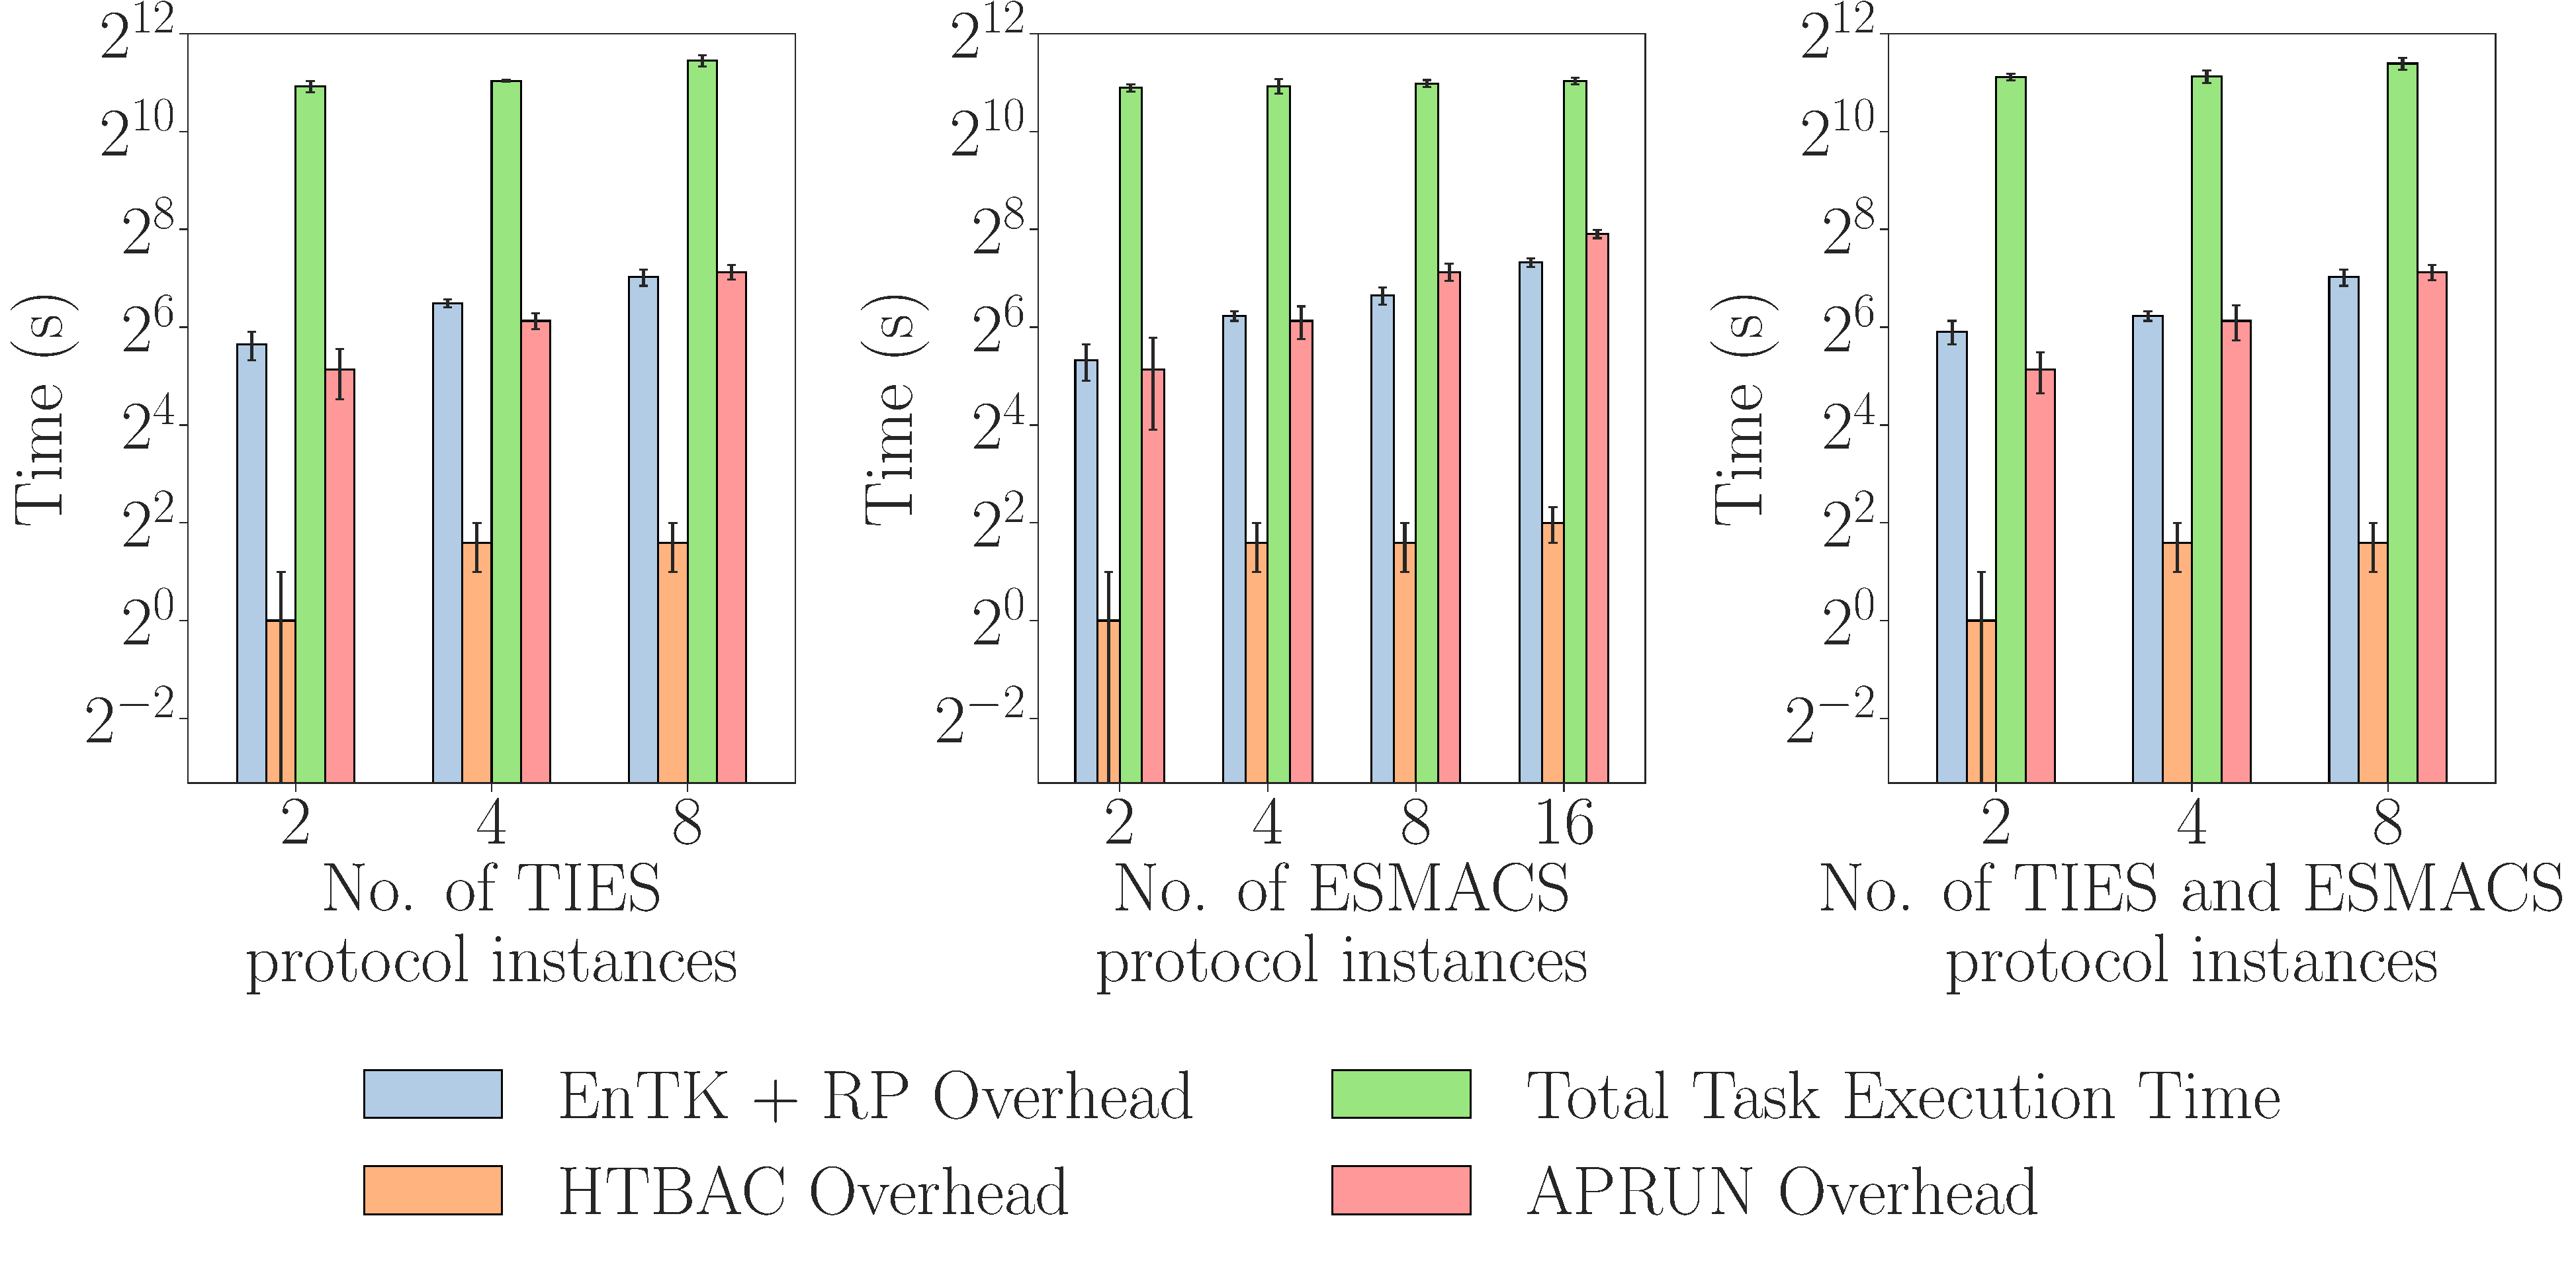
\includegraphics[width=\columnwidth]{figures/ws_all_base2.pdf}
    \caption{Weak scaling of HTBAC. The ratio number of protocol instances to
    resources is constant. Task Execution Time with and HTBAC, EnTK+RP,
    \texttt{aprun} overheads with (a) TIES (Experiment 1), (b) ESMACS
    (Experiment 2), and (c) TIES and ESMACS (Experiment 3).}\label{fig:ws}
\up{}
\up{}
\up{}
\end{figure}

Fig.~\ref{fig:ws}(b) shows the weak scaling of HTBAC with the ESMACS
protocol. We increase the number of instances linearly, between 2 and 16.
Each ESMACS protocol contains 1 pipeline with 4 stages and 25 concurrent
tasks.

Fig.~\ref{fig:ws}(c) shows the weak scaling of HTBAC with instances of both
TIES and ESMACS protocols. Also in this case, we scale the instances of both
protocols linearly, between 2 and 8. The first configuration shows 1 ESMACS
and 1 TIES protocol, and with each increase in scale we double the number of
protocols. Experiments 2 and 3 show scaling ranges within the limit of the
maximum number of concurrent tasks we can successfully execute on Blue
Waters.

For all weak scaling experiments (1--3) we use physical systems from the
\texttt{BRD4-GSK} library with the same number of atoms and similar chemical
properties. The uniformity of these physical systems ensures a consistent
workload with insignificant variability when characterizing their performance
under different conditions.

In all weak scaling experiments (Fig.~\ref{fig:ws}) we observe that the value
of Total Task Execution Time (green bar) shows minimal variation as the
number of protocol instances increases, suggesting that HTBAC is invariant to
the protocol. We conclude that HTBAC shows near-ideal weak scaling behavior
under these conditions.

The HTBAC overhead depends mostly on the number of protocol instances that
need to be generated for an application. This overhead shows a super linear
increase as we grow the number of protocol instances, but the duration of the
overhead is negligible when compared to Total Task Execution Time.

The \texttt{aprun} overhead increases as we approach the limit of concurrent
\texttt{aprun} processes that can be executed on Blue Waters. For example,
when scaling to 8 TIES protocol instances (Fig.~\ref{fig:ws}(a)), we see that
the increase in \texttt{aprun} overhead occurs due to task failure. This is
explained by noticing that attempts to relaunch failed tasks require
additional communication among the nodes that were running the tasks and the
MOM Nodes from which the execution is coordinated.

EnTK and RP overheads mostly depend on the number of tasks that need to be
translated in-memory from a Python object to a task
description~\cite{dakka2017,merzky2018}. As such, those overheads are
expected to grow proportionally to the number of tasks, as observed in
Fig.~\ref{fig:ws}, blue bars.

The RP overhead is calculated by measuring and aggregating the execution time
of the RP components that manage and coordinate the execution of the protocol
instances. Among these components, the task scheduler of RP introduces the
largest overhead. Due to the general scheduling algorithm loaded by default
in RP, the task scheduling overhead scales linearly with the number of tasks
that need to be scheduled.

In comparison to Total Task Execution Time, the EnTK and RP overheads are an
order of magnitude shorter, yet they directly contribute to the total
duration of the application execution. Based on Fig.~\ref{fig:ws}, we
approximate the use of our systems will results in $\approx15\%$ additional
usage of resource allocation. This overhead can be substantially reduced by
using a special-purpose scheduler for RP as illustrated in
Ref.~\cite{merzky2018}.

% C -------------------------------------------------------------------------
\subsection{Strong Scaling Characterization}

In Experiment 4 we fix the number of instances of the TIES protocol to 8 (due
to the described \texttt{aprun} limitations) and we vary the amount of
resources between 4160, 8320 and 16640 cores. Assuming the definition of
`generation' in \S\ref{ssec:exp_design}, given 4160 cores, we can execute 4
generations of 130 concurrent tasks; with 8320 cores, 2 generations of 260
tasks; and with 16640 cores, 1 generation of 520 tasks.

In Experiment 5 we fix the number of instances of the ESMACS protocols to 16
and vary the amount of resources between 3200, 6400 and 12800 cores. In this
way, we obtain the same number of generations as in Experiment 4.

In Experiment 6 we fix the number of instances of the ESMACS and TIES
protocols to 16 and 4 respectively, and vary the amount of resources between
5280, 10560 and 22120 cores. In this way, we obtain the same number of
generations as in Experiment 4 and 5.

Fig.~\ref{fig:ss} shows a linear speedup in Total Task Execution Time for
both experiments, proportional to the increase in the number of cores. The
availability of more resources for a fixed number of protocols explains this
behavior. Overheads remain essentially constant for both experiments when
increasing the number of cores. The scheduling of the number of tasks, as
opposed to the amount of resources, is the main driver of EnTK and RP
overheads (Ref.~\cite{merzky2018}).

\begin{figure}
  \centering
   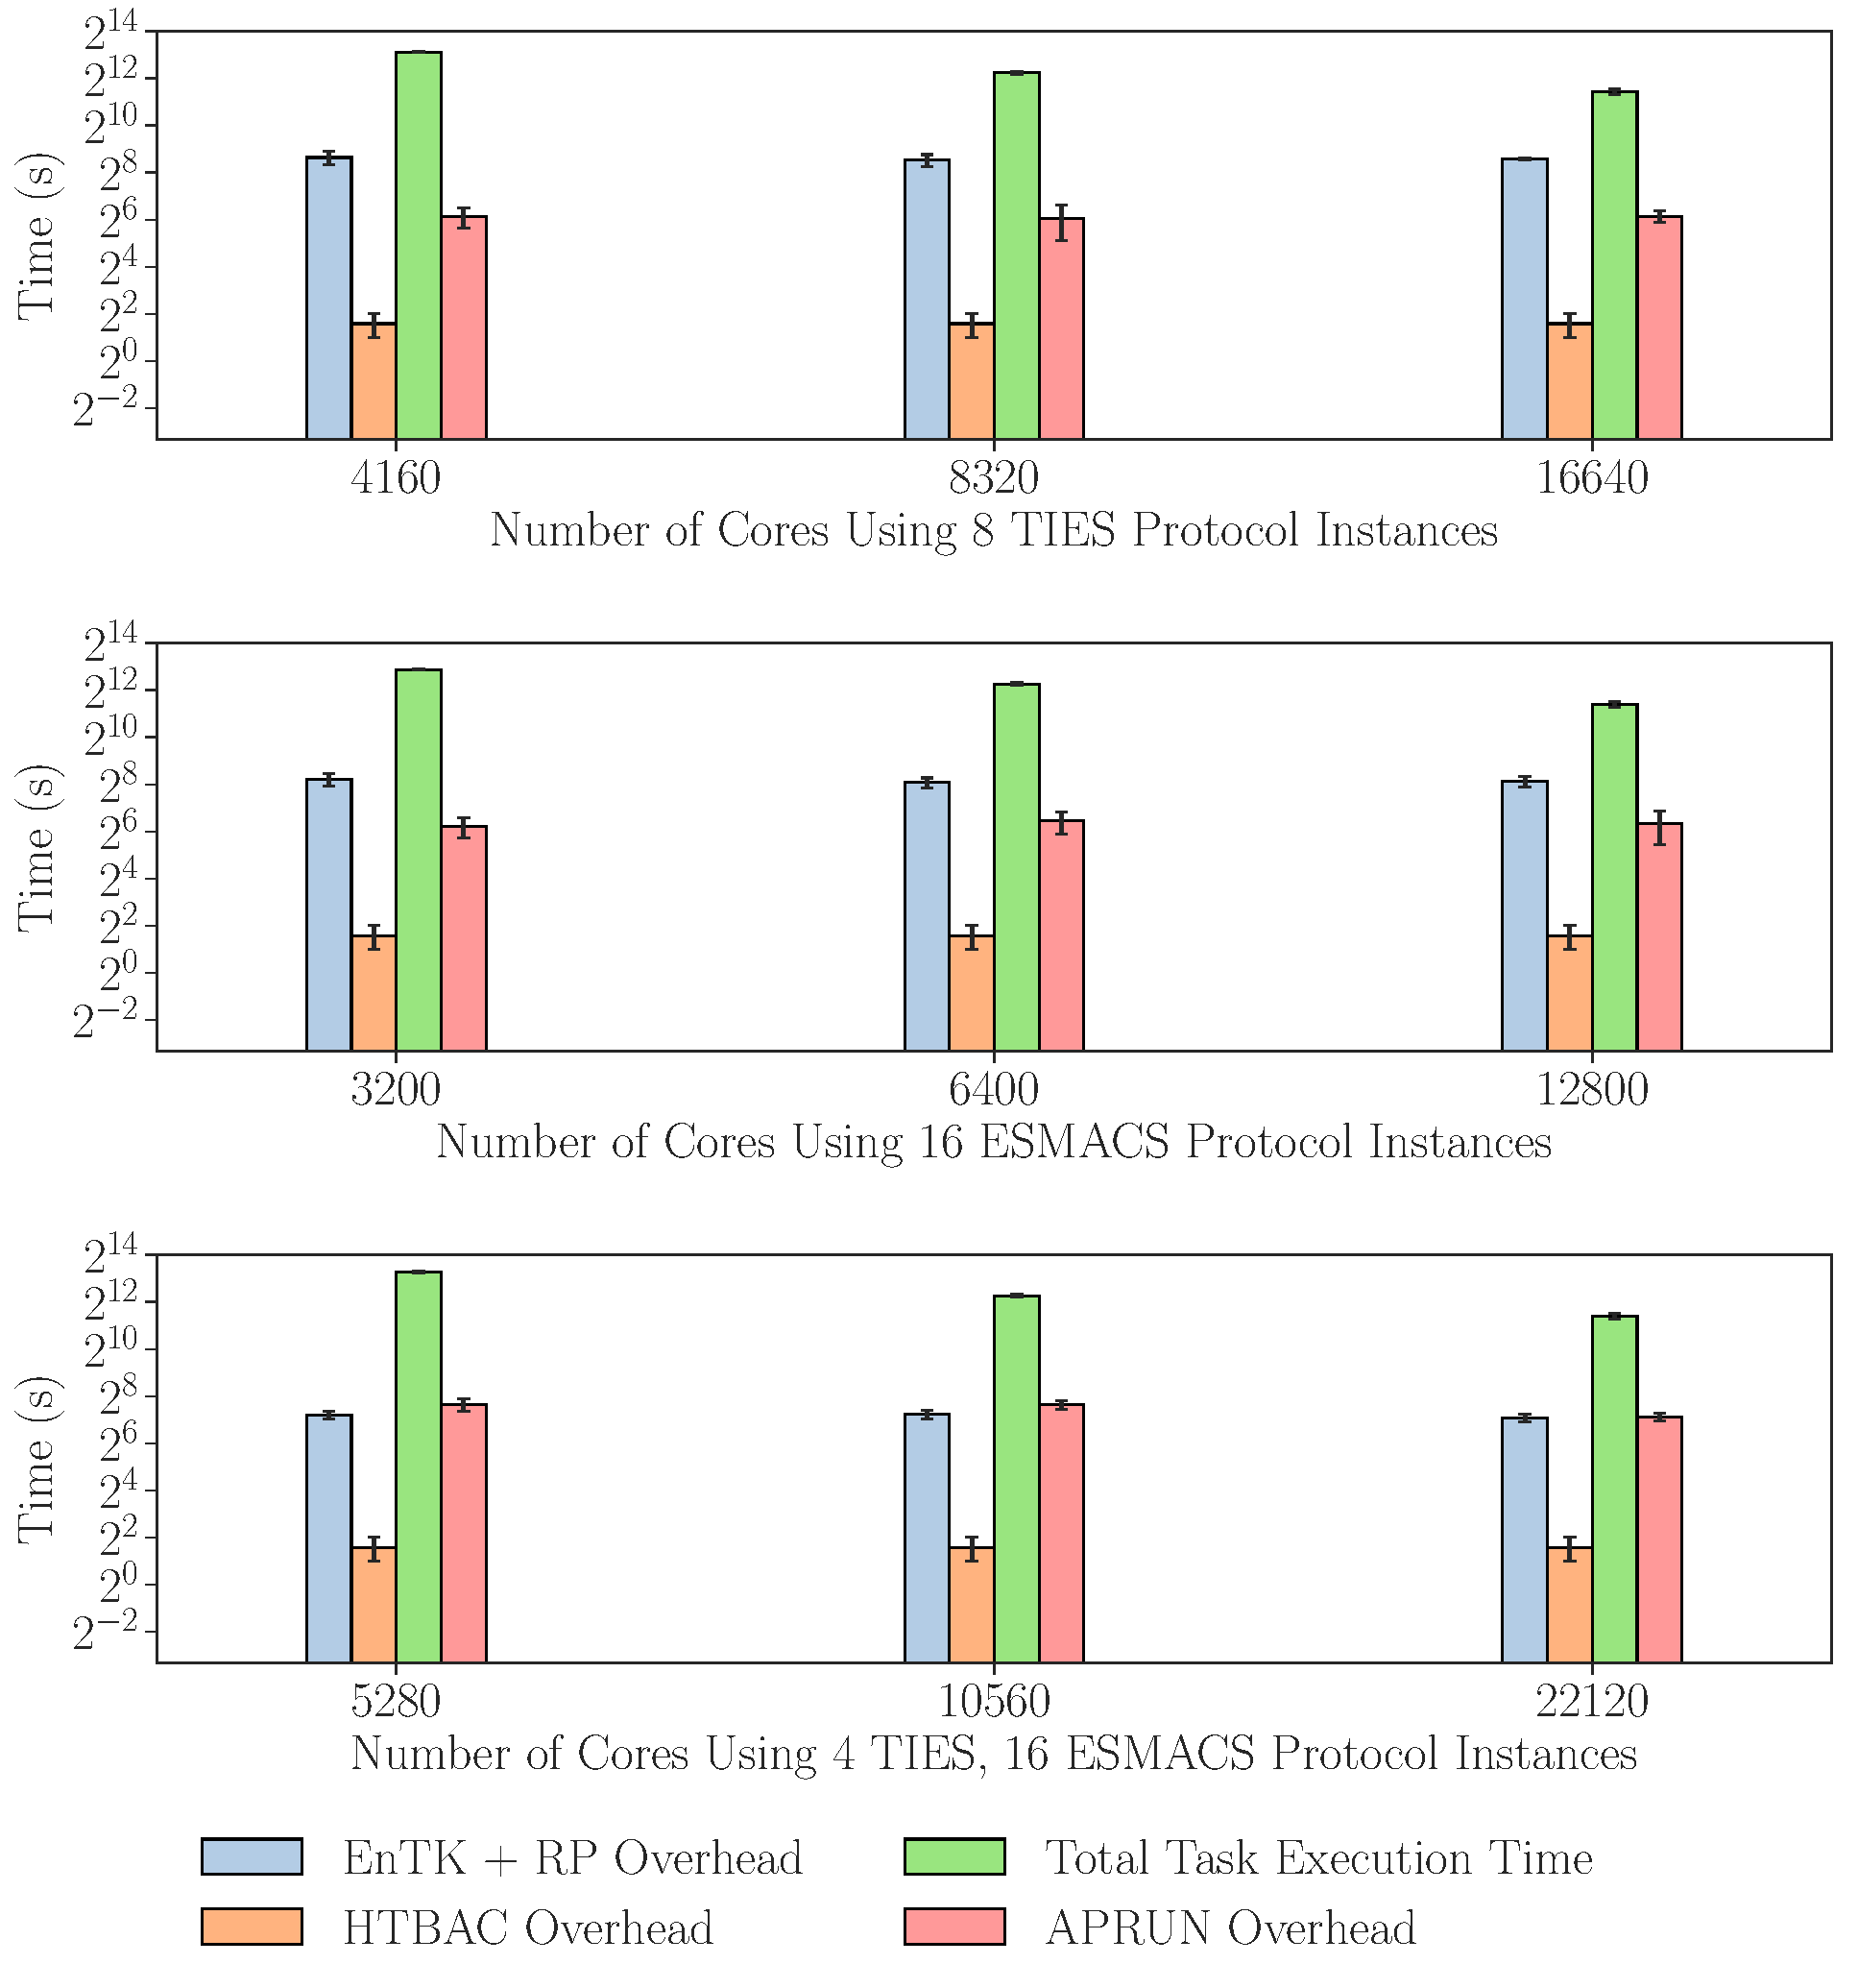
\includegraphics[width=\columnwidth]{figures/ss_all_base2.pdf}
   \caption{Strong scaling of HTBAC. The number of protocol instances is
    fixed while the number of core increases. Task Execution Time with and
    HTBAC, EnTK+RP, \texttt{aprun} overheads with (a) TIES (Experiment 4),
    ESMACS (Experiment 5) and ESMACS + TIES (Experiment 6).}\label{fig:ss}
\up{}
\up{}
\up{}
\end{figure}

% D -------------------------------------------------------------------------
\subsection{Validation}

In order to validate the correctness of the results produced in Experiment
1--6, using HTBAC and the BRD4-GSK physical systems, we compare our results
with those previously published in Wan et al.~\cite{Wan2017brd4}. In this
way, we can confirm that we calculated the correct binding free energies
values.

We validated our implementation selecting a subset of the protein ligand
systems used in Wan et al.~\cite{Wan2017brd4}: ligand transformations 3 to 1,
4, and 7. We then performed a full simulation on all 3 systems and calculated
the binding affinity using HTBAC.

The results of our experiments, collected in Table~\ref{tab:exp2}, show that
all three $\Delta \Delta$G values are within error bars of the original
study, validating the results we produced with HTBAC.

\begin{table}
  \centering
  \caption{Validation of HTBAC results against published and experimental
  values}\label{tab:exp2}  
  \begin{tabular}{lrrr}
    \toprule
    System & 
    {\makecell{HTBAC \\ (\si{\kilo\calorie\per\mole})}} & 
    {\makecell{Wan et al. \\ (\si{\kilo\calorie\per\mole})}} & 
    {\makecell{Experiment \\ (\si{\kilo\calorie\per\mole})}} \\
    \midrule
    BRD4 \textbf{3 to 1} & \num{0.39 +- 0.10} &   \num{0.41 +- 0.04} &  \num{0.3 +- 0.09} \\
    BRD4 \textbf{3 to 4} & \num{0.02 +- 0.12} &   \num{0.01 +- 0.06} &  \num{0.0 +- 0.13} \\
    BRD4 \textbf{3 to 7} & \num{-0.88 +- 0.17} &  \num{-0.90 +- 0.08} & \num{-1.3 +- 0.11} \\
    \bottomrule
  \end{tabular}
\up{}
\up{}
\up{}
\end{table}

% E -------------------------------------------------------------------------
\subsection{Adaptive Experiments}

The design of HTBAC permits enhancing protocols while continuing to use
``static'' simulation engines. To this end, we implemented two adaptive
methods using HTBAC: adaptive quadrature and adaptive termination. Both of
these methods use the features of adaptivity offered in HTBAC to scale to
large number of concurrent simulations and to increase convergence rate and
obtain more accurate scientific results.

The aim of introducing adaptive quadrature for alchemical free energy
calculation protocols (e.g., TIES) is to reduce time to completion while
maintaining (or increasing) the accuracy of the results. Time to completion
is measured by the number of core hours consumed by the simulations. Accuracy
is defined as the error with respect to a reference value, calculated via a
dense $\lambda$ window spacing (65 windows). This reference value is used to
establish the accuracy of the non-adaptive protocol (which has 13 $\lambda$
windows) and the adaptive protocol (which has a variable number of $\lambda$
windows, determined at run time).

One of the input parameters of the adaptive quadrature algorithm is the
desired acceptable error threshold of the estimated integral. We set this
threshold to the error of the non-adaptive algorithm calculated via the
reference value. The algorithm then tries to minimize the number of $\lambda$
windows constrained by the accuracy requirement.

\begin{figure}
  \begin{tikzpicture}
\begin{axis}[
  ybar,
  ymin=0,
  ylabel=Error (kcal/mol),
  x tick label style  = {text width=1.5cm,align=center},
  symbolic x coords={PTP1B L1-L2,PTP1B L10-L12,TYK2 L7-L8,TYK2 L4-L9,MCL1 L32-L38}
  ]
  
\addplot+[color=Orchid] table [x=System, y=Non-adaptive error, col sep=comma] {figures/savings.csv};

\addplot+[color=YellowGreen] table [x=System, y=Adaptive error, col sep=comma] {figures/savings.csv};


\legend{Non-adaptive,Adaptive}
  
\end{axis}
\end{tikzpicture}%
%
%
\begin{tikzpicture}
\begin{axis}[
  ybar,
  ymin=0,
  ylabel=Resource consumption (CPU-hours),
  x tick label style  = {text width=1.5cm,align=center},
  symbolic x coords={PTP1B L1-L2,PTP1B L10-L12,TYK2 L7-L8,TYK2 L4-L9,MCL1 L32-L38}
  ]
  
\addplot+[color=Orchid] table [x=System, y=Non-adaptive cpuh, col sep=comma] {figures/savings.csv};

\addplot+[color=YellowGreen] table [x=System, y=Adaptive cpuh, col sep=comma] {figures/savings.csv};


\legend{Non-adaptive,Adaptive}
  
\end{axis}
\end{tikzpicture}
%
  \caption{Quantifying the benefits of the adaptive quadrature simulations.
  (top) The error of the adaptive run is reduced for all 5 test systems,
  sometimes by a significant amount. It has been shown that reproducibility
  of free energy calculations can be achieved up to
  \SI{0.2}{\kilo\calorie\per\mole}~\cite{Loeffler2018}. The adaptive
  algorithm brings down the error of the nonadaptive simulations below this
  threshold, ensuring that results are also reproducible. (bottom) Resource
  consumption is reduced, except for one of the systems, where the low error
  threshold required more $\lambda$ windows.}\label{fig:savings}
\up{}
\up{}
\end{figure}

Table~\ref{tab:adapquad} shows the results of running adaptive quadrature on
5 protein ligand systems, comparing the Total Task Execution Time and
accuracy versus the non-adaptive case. The number of lambda windows are
reduced on average by \SI{32}{\percent}, hence reducing Total Task Execution
Time by the same amount. The error on the adaptive results is also decreased,
on average by \SI{77}{\percent} (see fig.~\ref{fig:savings}). More
importantly, the error on all of the systems are reduced to below
\SI{0.2}{\kilo\calorie\per\mole}, which has recently been shown to be the
upper bound of reproducibility across different simulation
engines~\cite{Loeffler2018}.

The Total Task Execution Time of the TYK2 L7--L8 system has increased for the
adaptive run by 1 $\lambda$ window, compared to the non-adaptive case. This
is due to the non-adaptive error being very low, and matching that same
accuracy required the use of a large number of windows. Nonetheless due to
the efficient placing of the windows, the accuracy of the free energy still
increased by \SI{40}{\percent}.

\begin{table*}
  \caption{Comparing results of adaptive, non-adaptive and reference
  runs.}\label{tab:adapquad}
  \begin{tabular}{lSSSSS[table-format=5.1]S[table-format=5.1]}
    \toprule
    {System}                               & 
    {\makecell{Ref $\Delta \Delta$G \\ (\si{\kilo\calorie\per\mole})}}  &
    {\makecell{Non-adaptive $\Delta \Delta$G \\ (\si{\kilo\calorie\per\mole})}}       &
    {\makecell{Adaptive $\Delta \Delta$G \\ (\si{\kilo\calorie\per\mole})}}           &
    {No. of $\lambda$ windows}            &
    {Decrease in TTX}       &
    {Increase in accuracy}                 \\
    \midrule
    {PTP1B L1-L2}   & 
    -58.51 & 
    -57.87(64) & 
    -58.60(9) & 
    10 & 
    23\si{\percent} & 
    86\si{\percent} \\
    %
    {PTP1B L10-L12} & 
    1.83   & 
    2.05(22) & 
    1.94(7)  & 
    6  & 
    54\si{\percent} &
    68\si{\percent} \\
    %
    {MCL1  L32-L38} & 
    2.13   & 
    2.33(20) & 
    2.14(1)      & 
    7  & 
    46\si{\percent} & 
    95\si{\percent} \\
    %
    {TYK2  L4-L9}   &
    -28.69 & 
    -28.25(44) & 
    -28.67(1)  & 
    7  & 
    46\si{\percent} & 
    98\si{\percent} \\
    %
    {TYK2  L7-L8}   & 
    4.97   & 
    4.92(5) & 
    5.00(3)      & 
    14 &  
    -8\si{\percent} & 
    40\si{\percent} \\
    \bottomrule 
  \end{tabular}
\end{table*}

Fig.~\ref{fig:adapconv} compares the error on the adaptive and non-adaptive
simulations as a time series plot. As fewer lambda windows are calculated the
adaptive algorithm uses less resources. Remarkably, the error is drastically
reduced as the windows are placed adaptively to capture the changes in
function.

\begin{figure}
  \begin{tikzpicture}
\begin{axis}[
  title style={align=center},
  title={Observed accuracy of adaptive vs. non-adaptive workflows\\for same simulation duration ({\SI{6}{\nano\second}}) },
  no markers,
  every axis plot/.append style={ultra thick},
  xlabel=Resource consumption (CPU-hours),
  ylabel=Error (kcal/mol),
  scaled ticks=false,
  yticklabel style={
  /pgf/number format/precision=3,
  /pgf/number format/fixed},
  scale=0.85,
  ]
  
  
\addplot+[color=Orchid, smooth] table [x=Resource consumption, y=Non-adaptive error, col sep=comma] {figures/non_adaptive_accuracy.csv};

\addplot+[color=YellowGreen, smooth] table [x=Resource consumption, y=Adaptive error, col sep=comma] {figures/adaptive_accuracy.csv};

\legend{Non-adaptive,Adaptive}

\draw[densely dotted, color=gray] (10586.058921984,0.049299384672436553) -- (12000,0.049299384672436553);
\draw[densely dotted, color=gray] (8143.1222476800012,0.0015858767437348931) -- (12000,0.0015858767437348931);

\draw[densely dotted, color=gray] (10586.058921984,0.08) -- (10586.058921984,-0.025);
\draw[densely dotted, color=gray] (8143.1222476800012,0.08) -- (8143.1222476800012,-0.025);
\draw[->] (10586.058921984,0.075) -- (8143.1222476800012,0.075) ;
\node[align = right] at (8700, 0.115) {Resource\\consumption\\decrease};

\node at (9200, 0.025) {\contour{white}{Error decrease}};
\draw[->] (11500,0.049299384672436553) -- (11500,0.0015858767437348931) ;


  
\end{axis}
\end{tikzpicture}

  \caption{Plot of the error estimate as a function of the resource
  consumption, comparing the adaptive and nonadaptive simulations. The error
  estimate converges for both simulations but the window placement of the
  adaptive simulation considerably lowered the error.}\label{fig:adapconv}
\up{}
\up{}
\end{figure}

Adaptive quadrature is specific to alchemical free energy calculations.
\emph{Adaptive termination}, the second adaptive method implemented in HTBAC,
offers dynamic termination for any simulation protocol that has as its aim
the prediction of an observable value. The protocol monitors the convergence
of the observable as the simulation progresses, and stops the execution when
a criterion has been met. Non-adaptive protocols usually have a predefined
simulation time, set based on the assumption that the simulation will
converge by that time. This means that in practical examples the simulation
might have converged before the predefined time interval.

In the original TIES protocol the production part of the simulation has to be
run for \SI{4}{\nano\second} and the results are analyzed thereafter. This
assumes that all systems need this simulation time for the results to
converge. In reality, certain systems could converge faster, therefore one
can terminate the simulation before the static \SI{4}{\nano\second} end. This
would lead to faster time to insight and less compute resources consumed.
Adaptive termination was implemented in HTBAC by having a checkpoint every
$\tau = \SI{0.5}{\nano\second}$ in the simulation. Fig.~\ref{fig:termination}
shows how the observable for a specific simulation changes as a function of
resource consumption. At every checkpoint the convergence is evaluated, and
the simulation is indeed terminated earlier than the non-adaptive protocol
would suggest. Table~\ref{tab:adapterm} shows results that the adaptively
terminated TIES protocol saves compute resources and reduces time to insight
on average by \SI{16}{\percent} for the physical systems tested.

\begin{figure}
  \begin{tikzpicture}
\begin{axis}[
  height=5cm,
  width=\columnwidth,
  every axis plot/.append style={ultra thick},
  xlabel=Resource consumption (CPU-hours),
  ylabel=$\Delta$G (kcal/mol),
  scaled ticks=false,
  yticklabel style={
  /pgf/number format/precision=3,
  /pgf/number format/fixed},
  xmin=3533.3975040000005,
  xmax=12000,
  ymax=4.85,
  ]
  
  
\addplot+[no markers, color=Orchid, smooth, error bars/.cd, y dir=both,y explicit, error mark=none, error bar style={draw=gray}] table [x=Resource consumption, y=dG, col sep=comma] {figures/adaptive-termination-begin.csv};

\addplot [only marks, mark=|, mark options={color = OliveGreen, mark size = 5pt, thick}] coordinates {(4416.746880000001,4.451008938594887) (5300.096256000001,4.490752904442608) (6183.445632000001,4.543730747316334) (7066.795008000001,4.5784909284966355) (7950.144384000001,4.586120549368642) (8833.493760000001,4.5843340530391075) (9716.843136000001,4.577994475375011) (10600.192512000001,4.571614686607193) };

\addplot+[densely dashed, semithick, no markers, color=Orchid, smooth, error bars/.cd, y dir=both,y explicit, error mark=none, error bar style={draw=gray}] table [x=Resource consumption, y=dG, col sep=comma] {figures/adaptive-termination-end.csv};

\legend{Observable, Checkpoint}

% \draw[densely dotted, color=gray] (10586.058921984,0.049299384672436553) -- (12000,0.049299384672436553);
% \draw[densely dotted, color=gray] (8143.1222476800012,0.0015858767437348931) -- (12000,0.0015858767437348931);
% 
\draw[densely dotted, color=gray] (7950.144384000001,4.8) -- (7950.144384000001,4.4);
% \draw[densely dotted, color=gray] (8143.1222476800012,0.08) -- (8143.1222476800012,-0.025);
% \draw[->] (10586.058921984,0.075) -- (8143.1222476800012,0.075) ;
% \node[align = right] at (8700, 0.115) {Resource\\consumption\\decrease};
% 
\node[align = right] at (6800, 4.7) {Adaptively\\terminated};

\draw[densely dotted, color=gray] (10600.192512000001,4.8) -- (10600.192512000001,4.4);

\node[align = right] at (9300, 4.5) {Non-adaptive\\protocol end};


% \draw[->] (11500,0.049299384672436553) -- (11500,0.0015858767437348931) ;
% 
  
\end{axis}
\end{tikzpicture}

  \caption{Plot of the free energy as a function of the resources consumed
  (hence simulation time). The adaptive termination algorithm checks the
  convergence of the observable every $\tau = \SI{0.5}{\nano\second}$ and if
  the threshold (\SI{0.01}{\kilo\calorie\per\mole}) has been met, terminates
  the simulation.}\label{fig:termination}
\end{figure}

\begin{table}
  \caption{Simulation time of non-adaptive and adaptively terminated runs for
  a given convergence criterion}\label{tab:adapterm}
  \centering
  \begin{tabular}{lSSS[table-format=5.1, table-column-width=2cm]}
    \toprule
    {System}                               & 
    {Non-adaptive}      &
    {Adaptive}          &
    {Decrease in TTX}       \\
    \midrule
    {PTP1B L10-L12} & 
    6.0\si{\nano\second}   & 
    5.0\si{\nano\second}   & 
    16.7\si{\percent} \\
    %
    {TYK2 L4-L9}   &
    6.0\si{\nano\second} & 
    5.5\si{\nano\second} & 
     8.3\si{\percent} \\
    %
    {TYK2 L7-L8}   & 
    6.0\si{\nano\second}  & 
    4.5\si{\nano\second} & 
    25.0\si{\percent} \\
    \bottomrule 
  \end{tabular}
\up{}
\up{}
\end{table}